The data we chose to work with was largely data provided by default through Coursera. We have tables of data corresponding to assignments, each of which may be submitted multiple times by a single student. Each submission is tracked with a  timestamp, submission number, and final score. For the midterm and final we have a single submission with timestamp and grade. This aggregate information is at the core of three of our views: {\bf Aggregate View}, {\bf Timescale View} and {\bf
Impact View}

In addition, for each exam we have a breakdown of questions, how many points each was worth, and what percentage of the students correctly answered the question. This information is used to generate
{\bf Exam View} and the comparisons for subviews. 

Finally, we have demographic information for each student. Due to privacy concerns, we generated this data automatically, from the statistics and parameters provided to us based on the actual student data. This random demographic data (gender, age, continent/country and background) is sufficient for us to provide a prototype, though further work would require more accurate data. This data is summarized in the {\bf Demographic View} 

Though all pieces of data are maintained in separate .csv files, the (anonymized) student id allows tracking of student information from one piece of data to the next. Though 65,000 students enrolled in the course, fewer than 27,000 ever watched a video. In the end, we have fewer than 4,000 students who submitted assignments half that number actually completed the course with a passing grade. 

\subsection{Design}
The core of the visualization provided are \emph{views} which switch out the main \emph{graph panel} to isolate different components of the course. To augment the abilities of the graph we provide 
\emph{background computation} to isolate \emph{clusters} of students and \emph{impact} of components. As a fine-grained means of selection, we allow the instructor to superimpose \emph{filters} over the data.


\begin{figure}[htb]
 \centering
 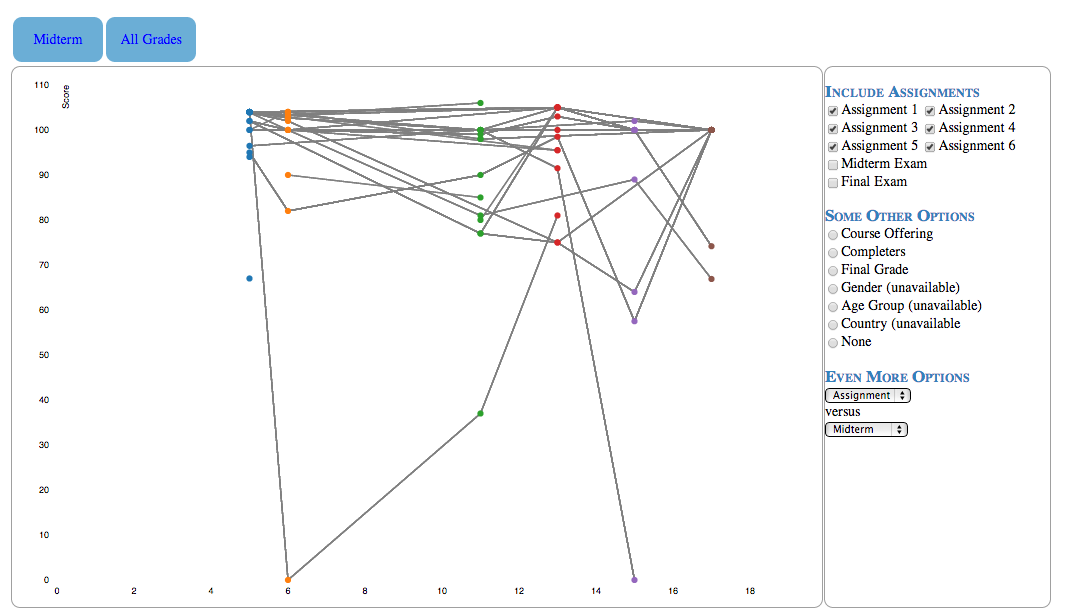
\includegraphics[width=3.5in]{aggregate_stub.png}
 \caption{Aggregate View.}
 \label{fig:aggregate}	
\end{figure}

\paragraph{Aggregate View (see Figure~\ref{fig:aggregate}) }
This view provides a generalized timescale view of the course. Each assignment and exam is represented as a point on the x axis, with grades represented (in percent) on the y axis. This view highlights the retention rate of the class, particularly when clusters are enabled. 


\begin{figure}[htb]
 \centering
 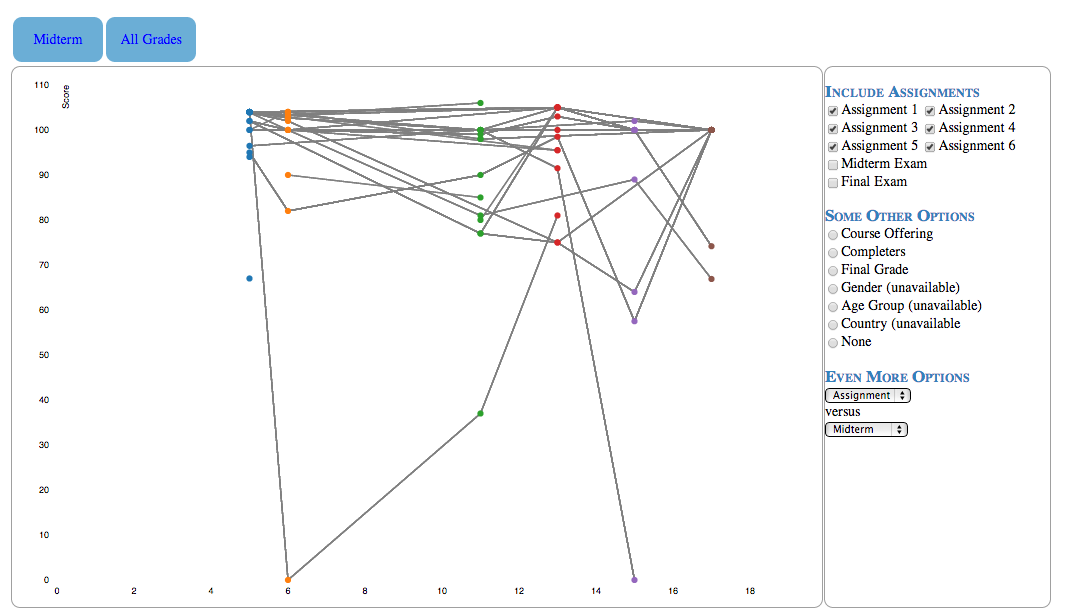
\includegraphics[width=3.5in]{aggregate_stub.png}
 \caption{Timescale View.}
 \label{fig:timescale}	
\end{figure}

\paragraph{Timescale View (see Figure~\ref{fig:timescale}) }
This view provides a zoomed-in view of the assignments and exam scores in relation to the timestamp with which they were submitted. This view originated from a desire to answer the question \emph{do late submitters overall score worse than early submitters?}


\begin{figure}[htb]
 \centering
 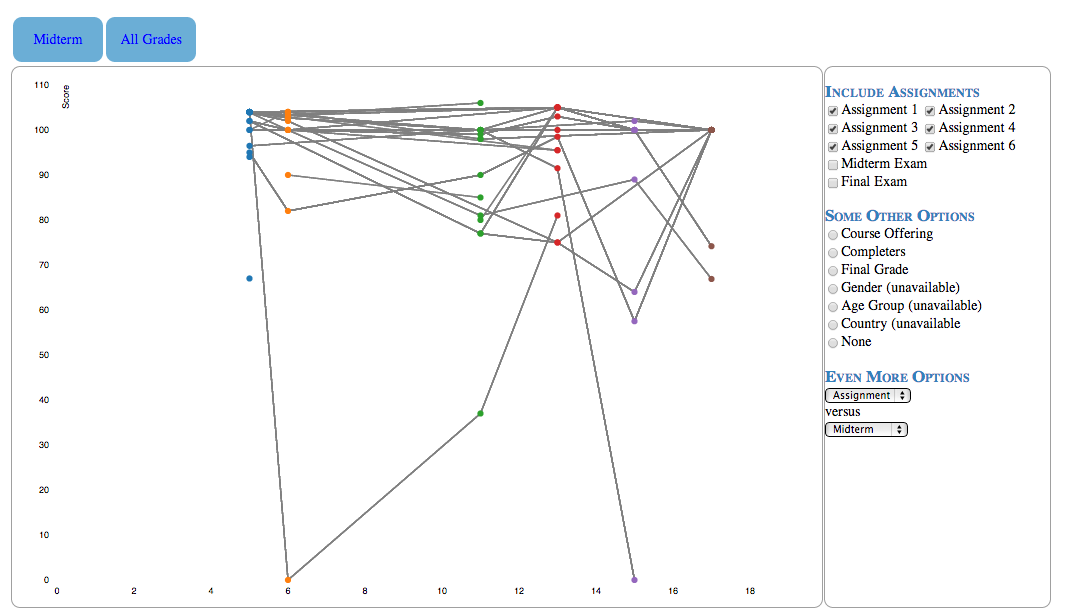
\includegraphics[width=3.5in]{aggregate_stub.png}
 \caption{Impact View.}
 \label{fig:impact}	
\end{figure}

\paragraph{Impact View (see Figure~\ref{fig:impact})}
This view provides a scatterplot reflecting the impact of an assignment or exam on the final grade. Each point is a single student, where the x value is the assignment grade and the y value is the final exam grade. In an ideal world, each assignment would be an equally good predictor of the final grade. When an assignment is a poor predictor, whether a student does well on that exam has little to no impact on the final grade, and we see a randomized scatter plot. When an assignment is a perfect predictor, we see a perfect diagonal formed by the scatter plot. Most assignments fall somewhere between the two.


\begin{figure}[htb]
 \centering
 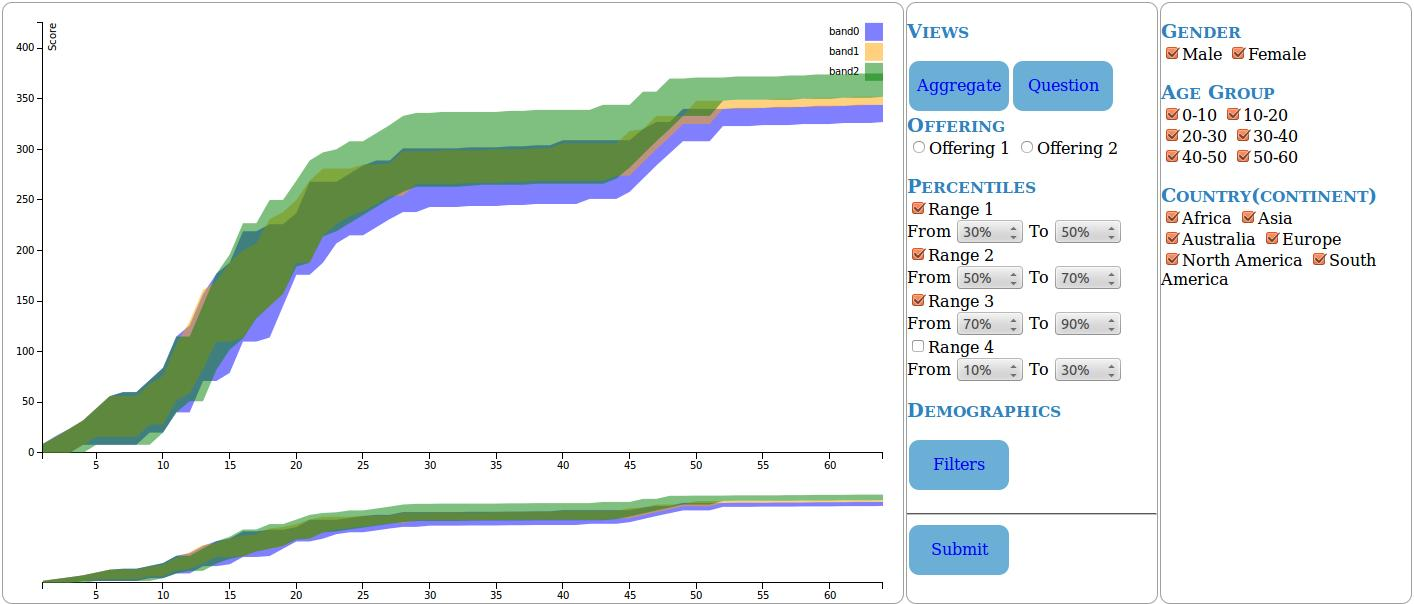
\includegraphics[width=3.5in]{Midterm_Final_Aggregate.jpeg}
 \caption{Comparing Midterm Scores in Aggregate. The exam progresses to the right, and we see the fan-out of scores between percentiles as students diverge in point value. }
\label{fig:exam1}	
\end{figure}

\begin{figure}[htb]
 \centering
 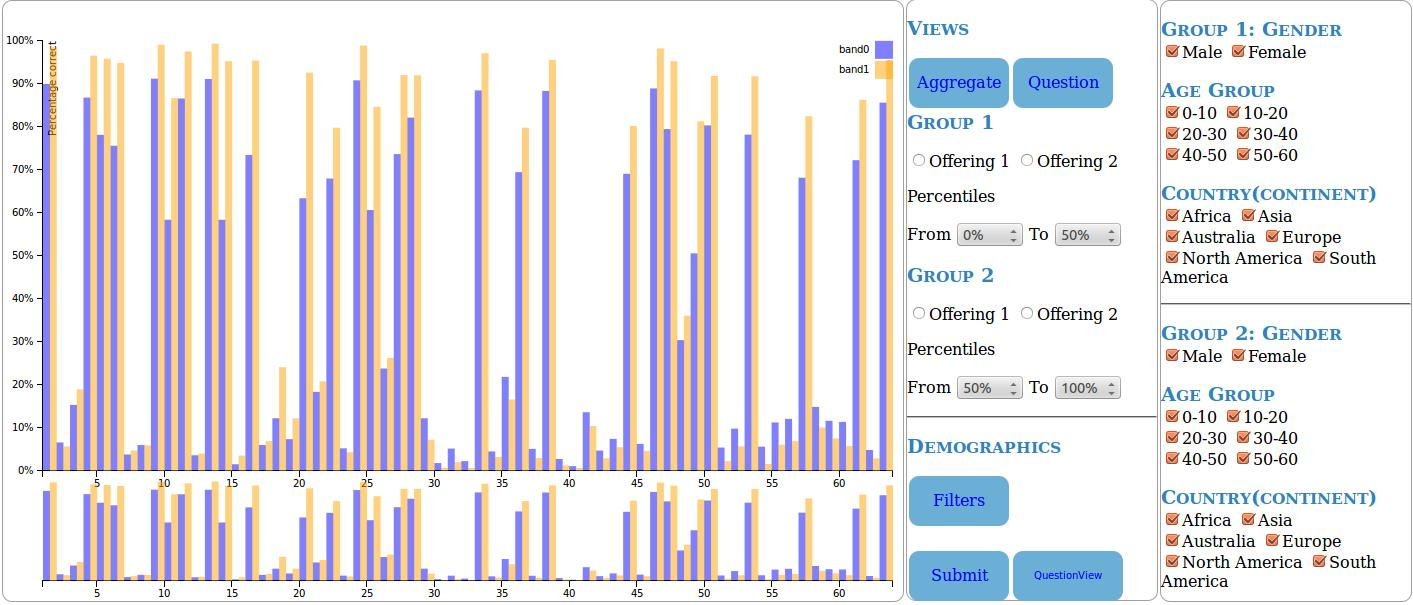
\includegraphics[width=3.5in]{Midterm_Final_Compare.jpeg}
 \caption{Comparing Midterm Scores Across Offerings }
\label{fig:exam2}	
\end{figure}

\begin{figure}[htb]
 \centering
 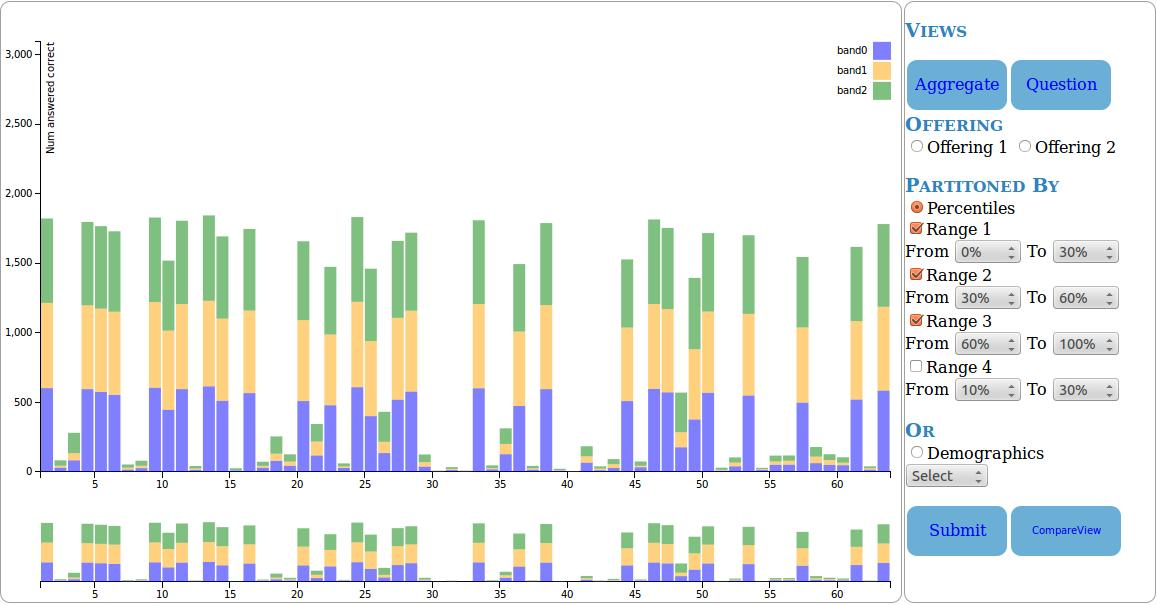
\includegraphics[width=3.5in]{Midterm_Final_Questions.jpeg}
 \caption{Comparing Midterm Questions by Student Percentile. }
\label{fig:exam3}	
\end{figure}

\paragraph{Exam View (see Figure~\ref{fig:exam1})}
TODO


\begin{figure}[htb]
 \centering
 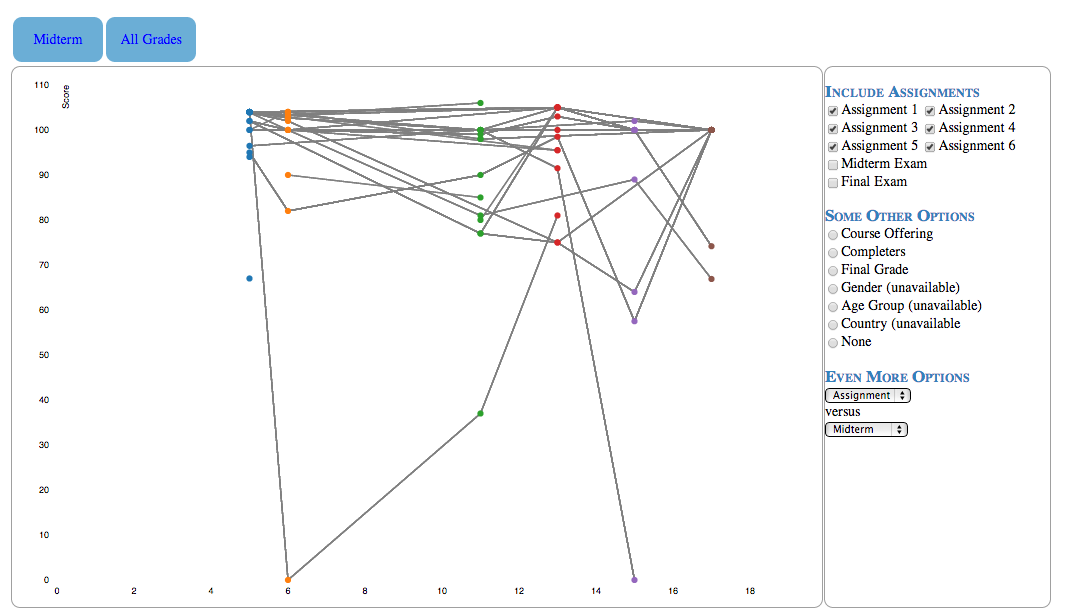
\includegraphics[width=3.5in]{aggregate_stub.png}
 \caption{Demographic View.}
  \label{fig:demo}	
\end{figure}

\paragraph{Demographic View (see Figure~\ref{fig:demo})}
TODO

\subsection{Background Computation}
To save time in loading the actual visualization, some of the computation is done in the background. 

\paragraph{Clustering}
Clusters are precomputed with a script (which must be run prior to the site being launched) and stored in data files for loading 
when requested. Given the quantity of data being processed, this significantly improves the responsiveness for a given page. 
These clusters are computed where the grades of each student (for all time or an exam) are considered a vector, and kmeans 
clustering is applied over the vector, with the distance function being a simple function over each vector pair:
\[  \sqrt{ (a_1-b_1)^2 + (a_2-b_2)^2 .... (a_n-b_n)^2   }\]

\paragraph{Impact}
The course element which most closely predicts the final grade is also precomputed and stored, using the same function above, this time with each assignment being a vector (of which each student is a dimension). However, for the actual display, though we default to the closest predictor (that with the closest distance and/or highest impact), each grade can be displayed without significant computation. Again, pre-computation of the distances saves significantly on load time. 
